%!TEX root=../cvFioretto.tex
%%%%%%%%%%%%%%%%%%%%%%%%%%%%%%%%%%%%%%%%%
% CV Fioretto
% Projects (long)
%	DCOPs for smart grids
%	DCOPs and GPUs
%	System Biology
%%%%%%%%%%%%%%%%%%%%%%%%%%%%%%%%%%%%%%%%%

%----------------------------------------------------------------------------------------
%	DCOP on Devices
%----------------------------------------------------------------------------------------
\begin{rSubsection}{Distributed Solutions for Smart Cities and Home Automation with DCOPs
%DCOP on Devices for Smart Grid Scheduling Problems
}{\em 2015 -- Present}{}{}
\item[]
\begin{figwindownonum}[0,l,{\mbox{%
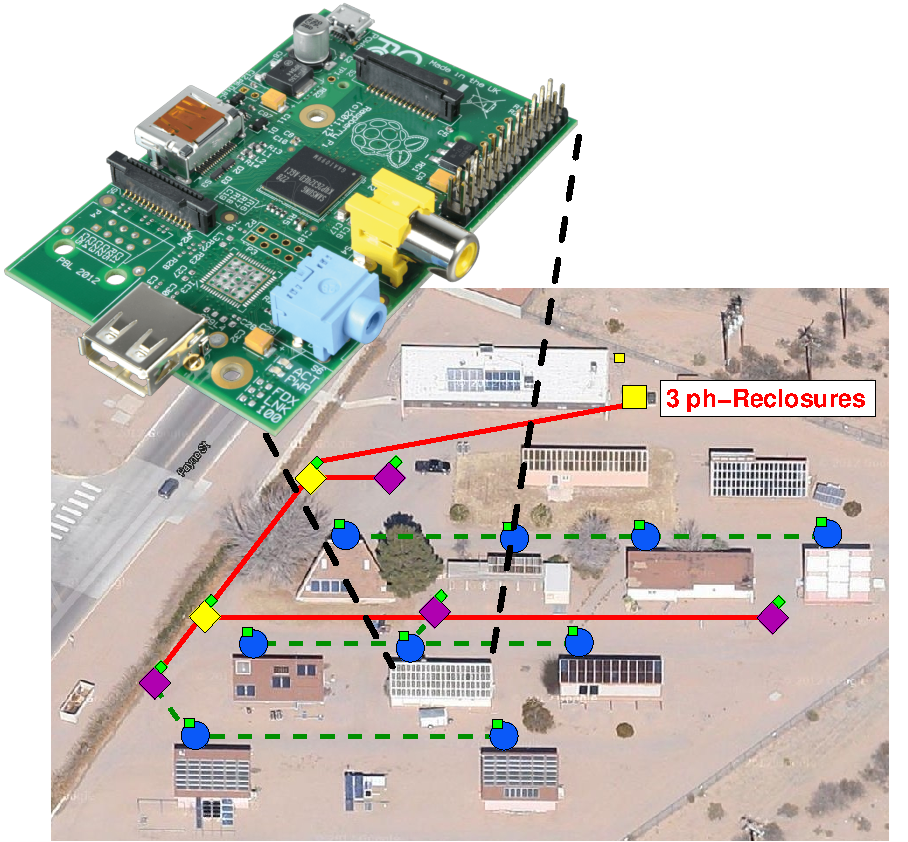
\includegraphics[width=140pt]{include/img/smart-grid}}},{~}]
%
In the context of smart grids, a challenging task is that of designing smart buildings that are capable of making autonomous decisions to control power productions, loads and transmissions. In this project we model residential and commercial buildings as autonomous agents, each of which is equipped with a small electronic device, able to monitor usage and production data, control the activation of several appliances, and store or consume energy from accumulators.
Agents will act cooperatively to reduce their consumptions costs as well as to ensure reliable and efficient energy delivery. 
The characteristics of the hardware adopted, as well as, the unpredictability of the available bandwidth motivate the development of new DCOP algorithms which work well under such constraints. The proposed algorithms are being deployed and evaluated on realistic smart buildings, within a \emph{micro-grid}.
%
%\item Two articles in preparation will be submitted to upcoming AI conferences.
\end{figwindownonum}
\end{rSubsection}

\vspace{-20pt}
%----------------------------------------------------------------------------------------
%	GPUs
%----------------------------------------------------------------------------------------
\begin{rSubsection}{GPU-accelerated Algorithms for Centralized and Distributed Optimization
%Speeding up Offline (D)COP Resolution with GPUs
}{2014 -- Present}{}{}
\item[]
\begin{figwindownonum}[0,l,{\mbox{%
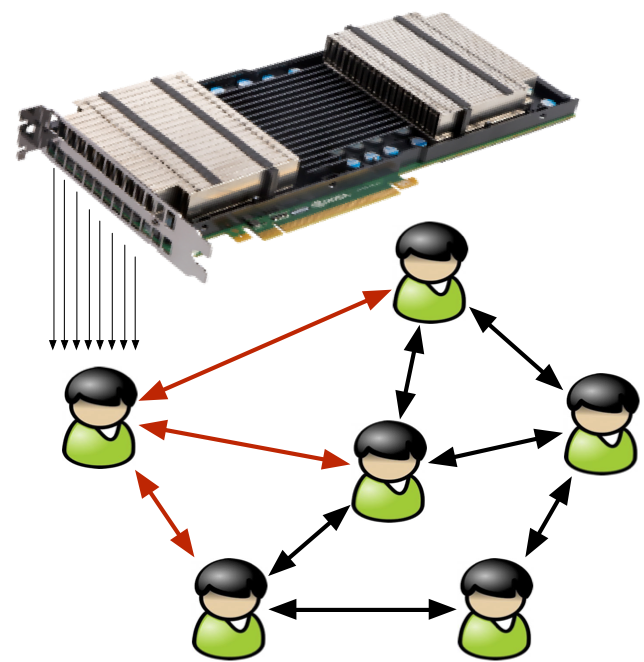
\includegraphics[width=140pt]{include/img/gpu-dcop}}},{~}]
%
GPU-accelerated computing is the use of a graphics processing unit (GPU) together with a CPU to accelerate general purpose applications. GPUs provide thousands of computing cores, %performing computations according to the Single Instruction Multiple Thread (SIMT) parallel paradigm. 
offering unprecedented application performance by offloading compute-intensive portions of the application to the GPU. \\
We have used GPUs to speedup inference-based and sampling-based optimization algorithms. The commonality of the former approaches is that, agents operate by replacing a variable and its related utility functions with a single new function, derived by optimizing over the possible values of the removed variable. Computing the new function can be decomposed in many independent operations, which makes inference-based (D)COP highly amenable to be parallelized on GPUs. 
The latter approaches have been accelerated with GPUs in the context of agents controlling multiple variables. Due to the stochastic nature of the sampling process, we adopted GPUs to perform a large number of parallel samples, resulting in faster algorithm convergence.
%
%\item One article in preparation will be submitted to upcoming AI conferences.
\end{figwindownonum}
\end{rSubsection}

\vspace{-20pt}
%----------------------------------------------------------------------------------------
%	System Biology and Constraints
%----------------------------------------------------------------------------------------
\begin{rSubsection}{Applied Constraint Programming in Computational Biology}{2012 -- 2015}{}{}
\item[]
\begin{figwindownonum}[0,l,{\mbox{%

\includegraphics[width=140pt]{include/img/dna}}},{~}]
Computational Biology is a wide field of study which involves subjects as the study of Proteins Structure and of Gene Regulatory Networks. A Gene Regulatory Networks (GRN) is a collection of DNA segments in a cell which interact with each other either directly or indirectly (through their RNA and protein expression products). Understanding the behavior of GRNs is a core interest in computational biology and medicine, as it is closely related with the process of drug production and assessment. We have employed committee machines to predict GRNs, and augment them with biologically meaningful constraints to filter irrelevant solutions. \\
Proteins are the product of coding genes, and perform a vast number of functions within living organisms. Their function is strictly related with their spatial conformation, therefore the Protein Structure Prediction (PSP) problem---which aims at predicting the 3D structure of a protein given its amino acid composition---is of central importance. 
We have developed a specialized Constraint Solver for the PSP problem, which employs efficient constraint propagators to search on the space of meaningful structures.
\end{figwindownonum}
\end{rSubsection}
\vspace{-20pt}
